\documentclass[e4_tp1_main.tex]{subfiles}

\begin{document}

\section{Ejercicio 3}

Se procedi\'o a integrar lo desarrollado en el ejercicio 1 con el ejercicio 2, switcheando la fuente buck con el circuito de disparo estudiado. 

\subsection{Curvas del convertidor buck}

En la figura \ref{fig:curvas3} observamos c\'omo la presencia del switch ``real'' afecta variables internas de la fuente. En primer lugar, los tiempos de conmutaci\'on del MOS son visibles en el gr\'afico, en comparaci\'on con la curva ideal. Sus efectos se ven claramente en el resto de las curvas: en $v_L$ se observa que le duty efectivo obtenido es superior a cuando se utiliz\'o el switch ideal. En efecto, la salida en este caso es de $V_O\simeq3.71V$, lo cual es consistente con tener un duty mayor.

A su vez, esto provoca que la corriente de la bobina tenga pendiente positiva por m\'as tiempo, lo cual explica el delay que se observa entre las curvas con llave ideal y real. Se observa tambi\'en que la corriente media es mayor con la llave real, lo cual es consistente con tener una tensi\'on de salida, y por lo tanto una corriente de salida, mayor.

En cuanto al diodo, volvemos a observar que conmuta m\'as tarde por el aumento del duty, pero adem\'as en este caso los picos de inversa son acotados: llegan a un m\'aximo de $I_{rr}=1.84$A.

\begin{figure}[ht]
	\centering
	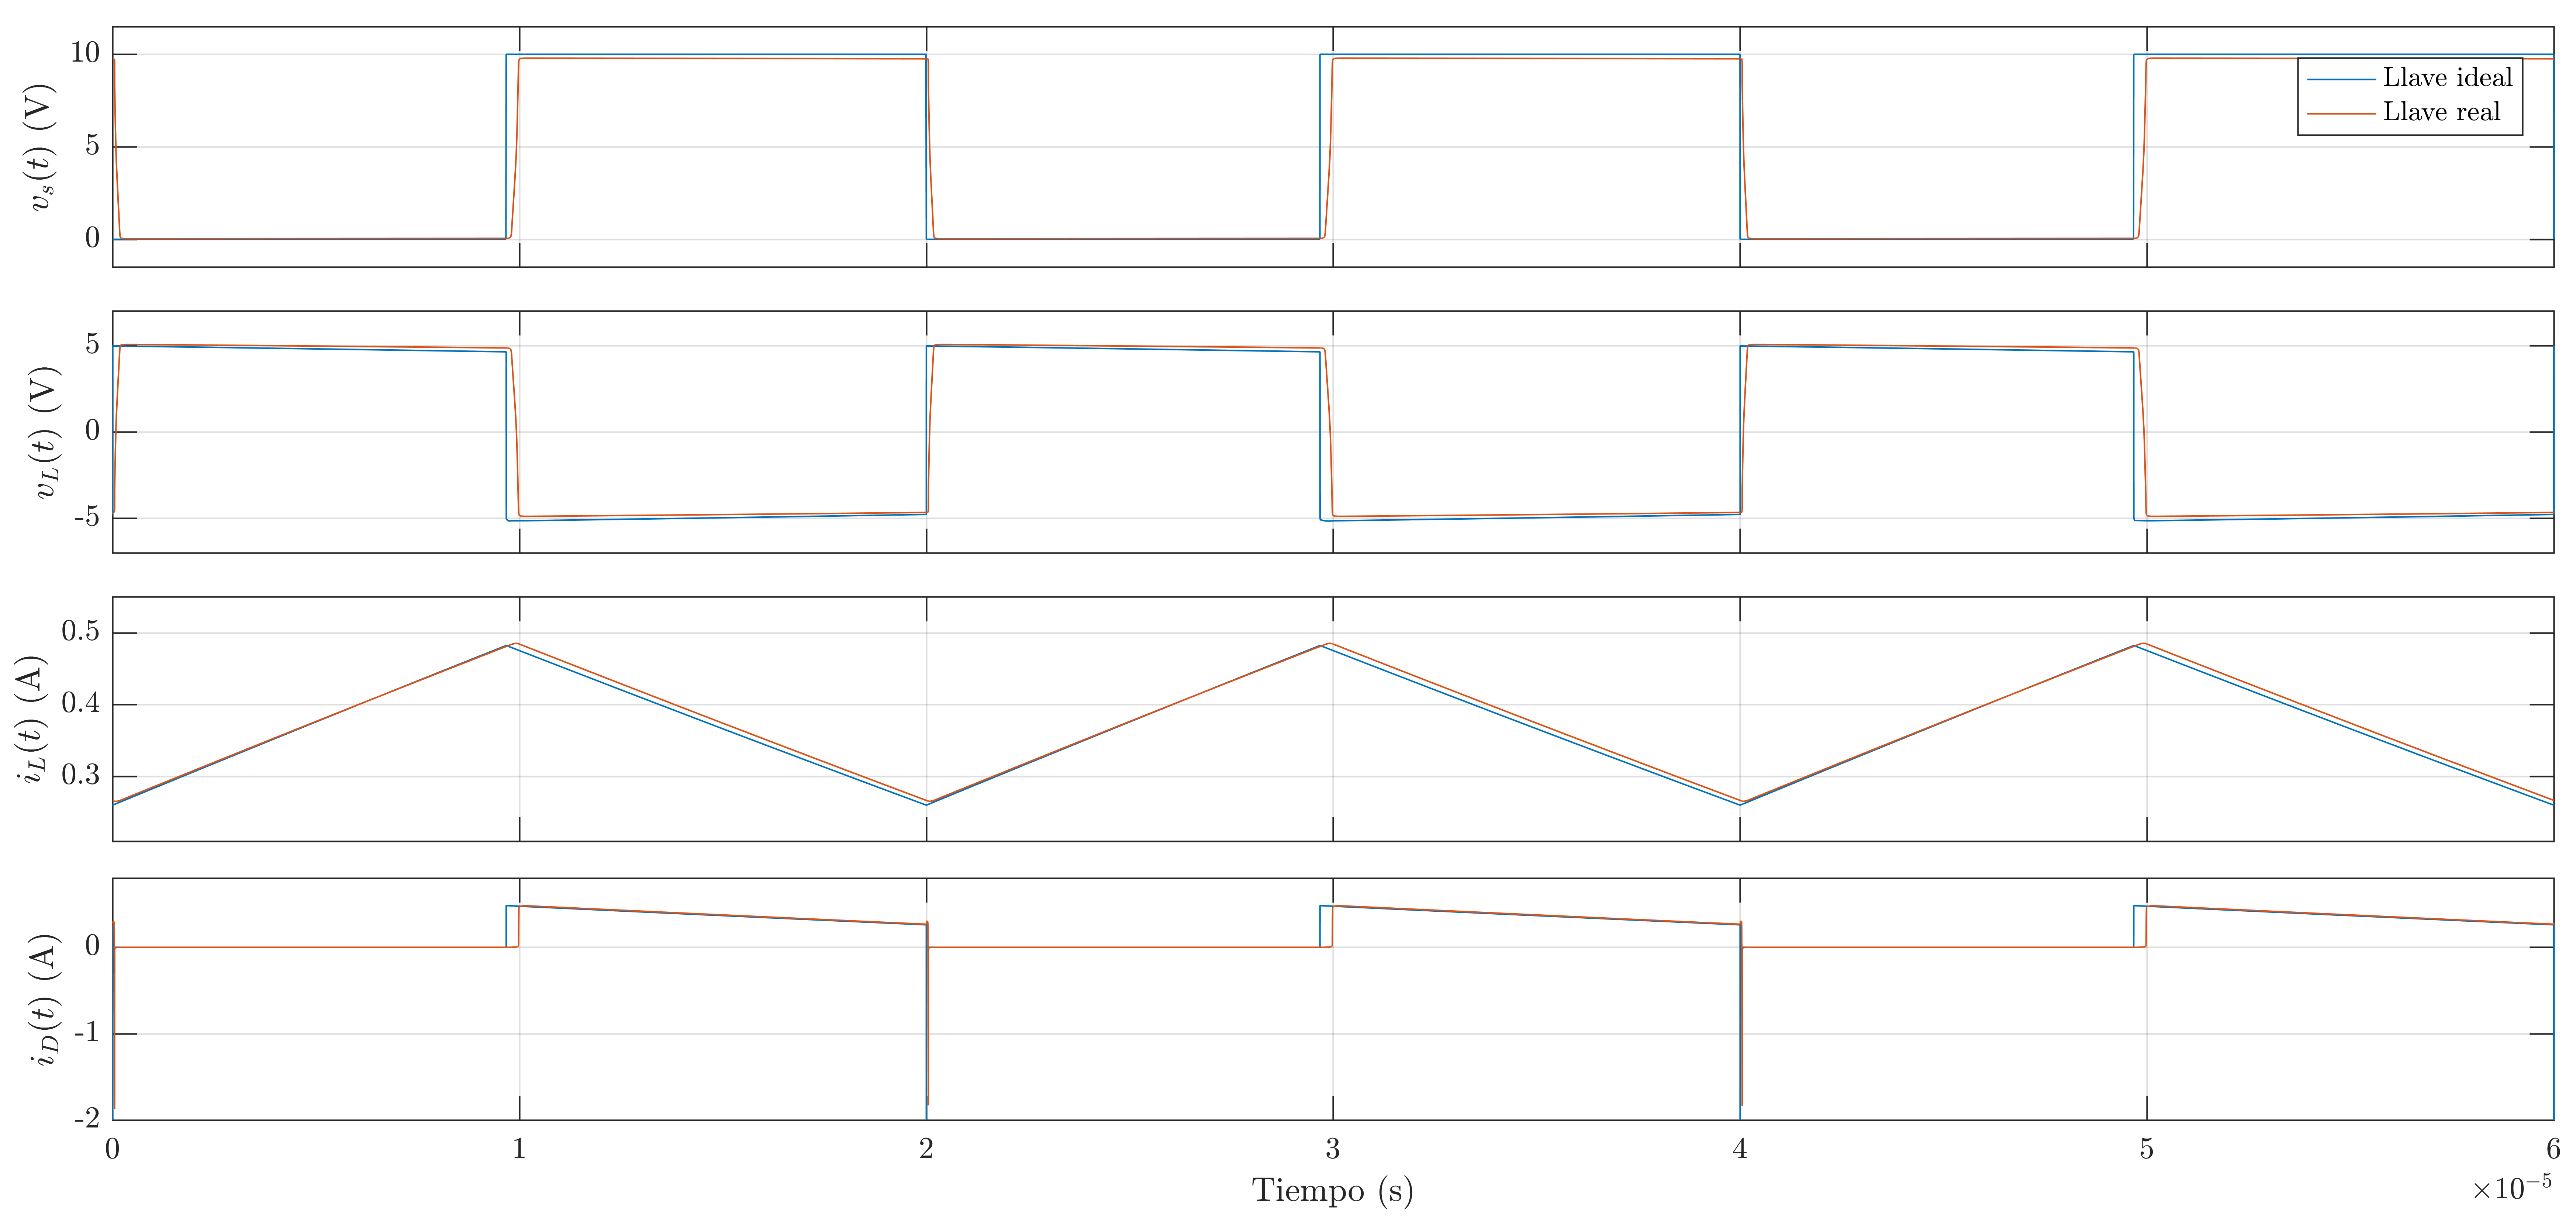
\includegraphics[width=0.75\textwidth]{images/ej3/curvas3.png}
	\caption{Curvas simuladas de la fuente buck con llave ideal y con llave real: de arriba hacia abajo, tensi\'on en la llave, tensi\'on en la bobina, corriente en la bobina, y corriente en el diodo.}
	\label{fig:curvas3}
\end{figure}

\subsection{Curvas de conmutaci\'on}

En cuanto a la conmutación, como se menciono previamente hay una clara diferencia entre los tiempo de conmutación. Esto es debido a las diferencias presentadas en la tensiones y las corrientes, generando valores de capacitancia menores a los que posee sin la Buck. Debido a que las capacitancias son menores es necesario una menor cantidad de carga y como los tiempos de rise y fall de corriente son proporcionales a las capacitancias, terminamos con tiempos de conmutación más chicos. Cabe mencionar que también debido a que las  tensiones entre $V_{g,io}$ y $V_{g,th}$ son más cercanas la variación de carga es también menor causando que los tiempos de rise y fall de tensión sean menores. 

Concluyendo, debido a los efectos que causan las diferencias de tensión y corriente entre ambos casos tenemos una disminución significativa de los tiempos de conmutación.




	\begin{figure}[ht]
		\centering
		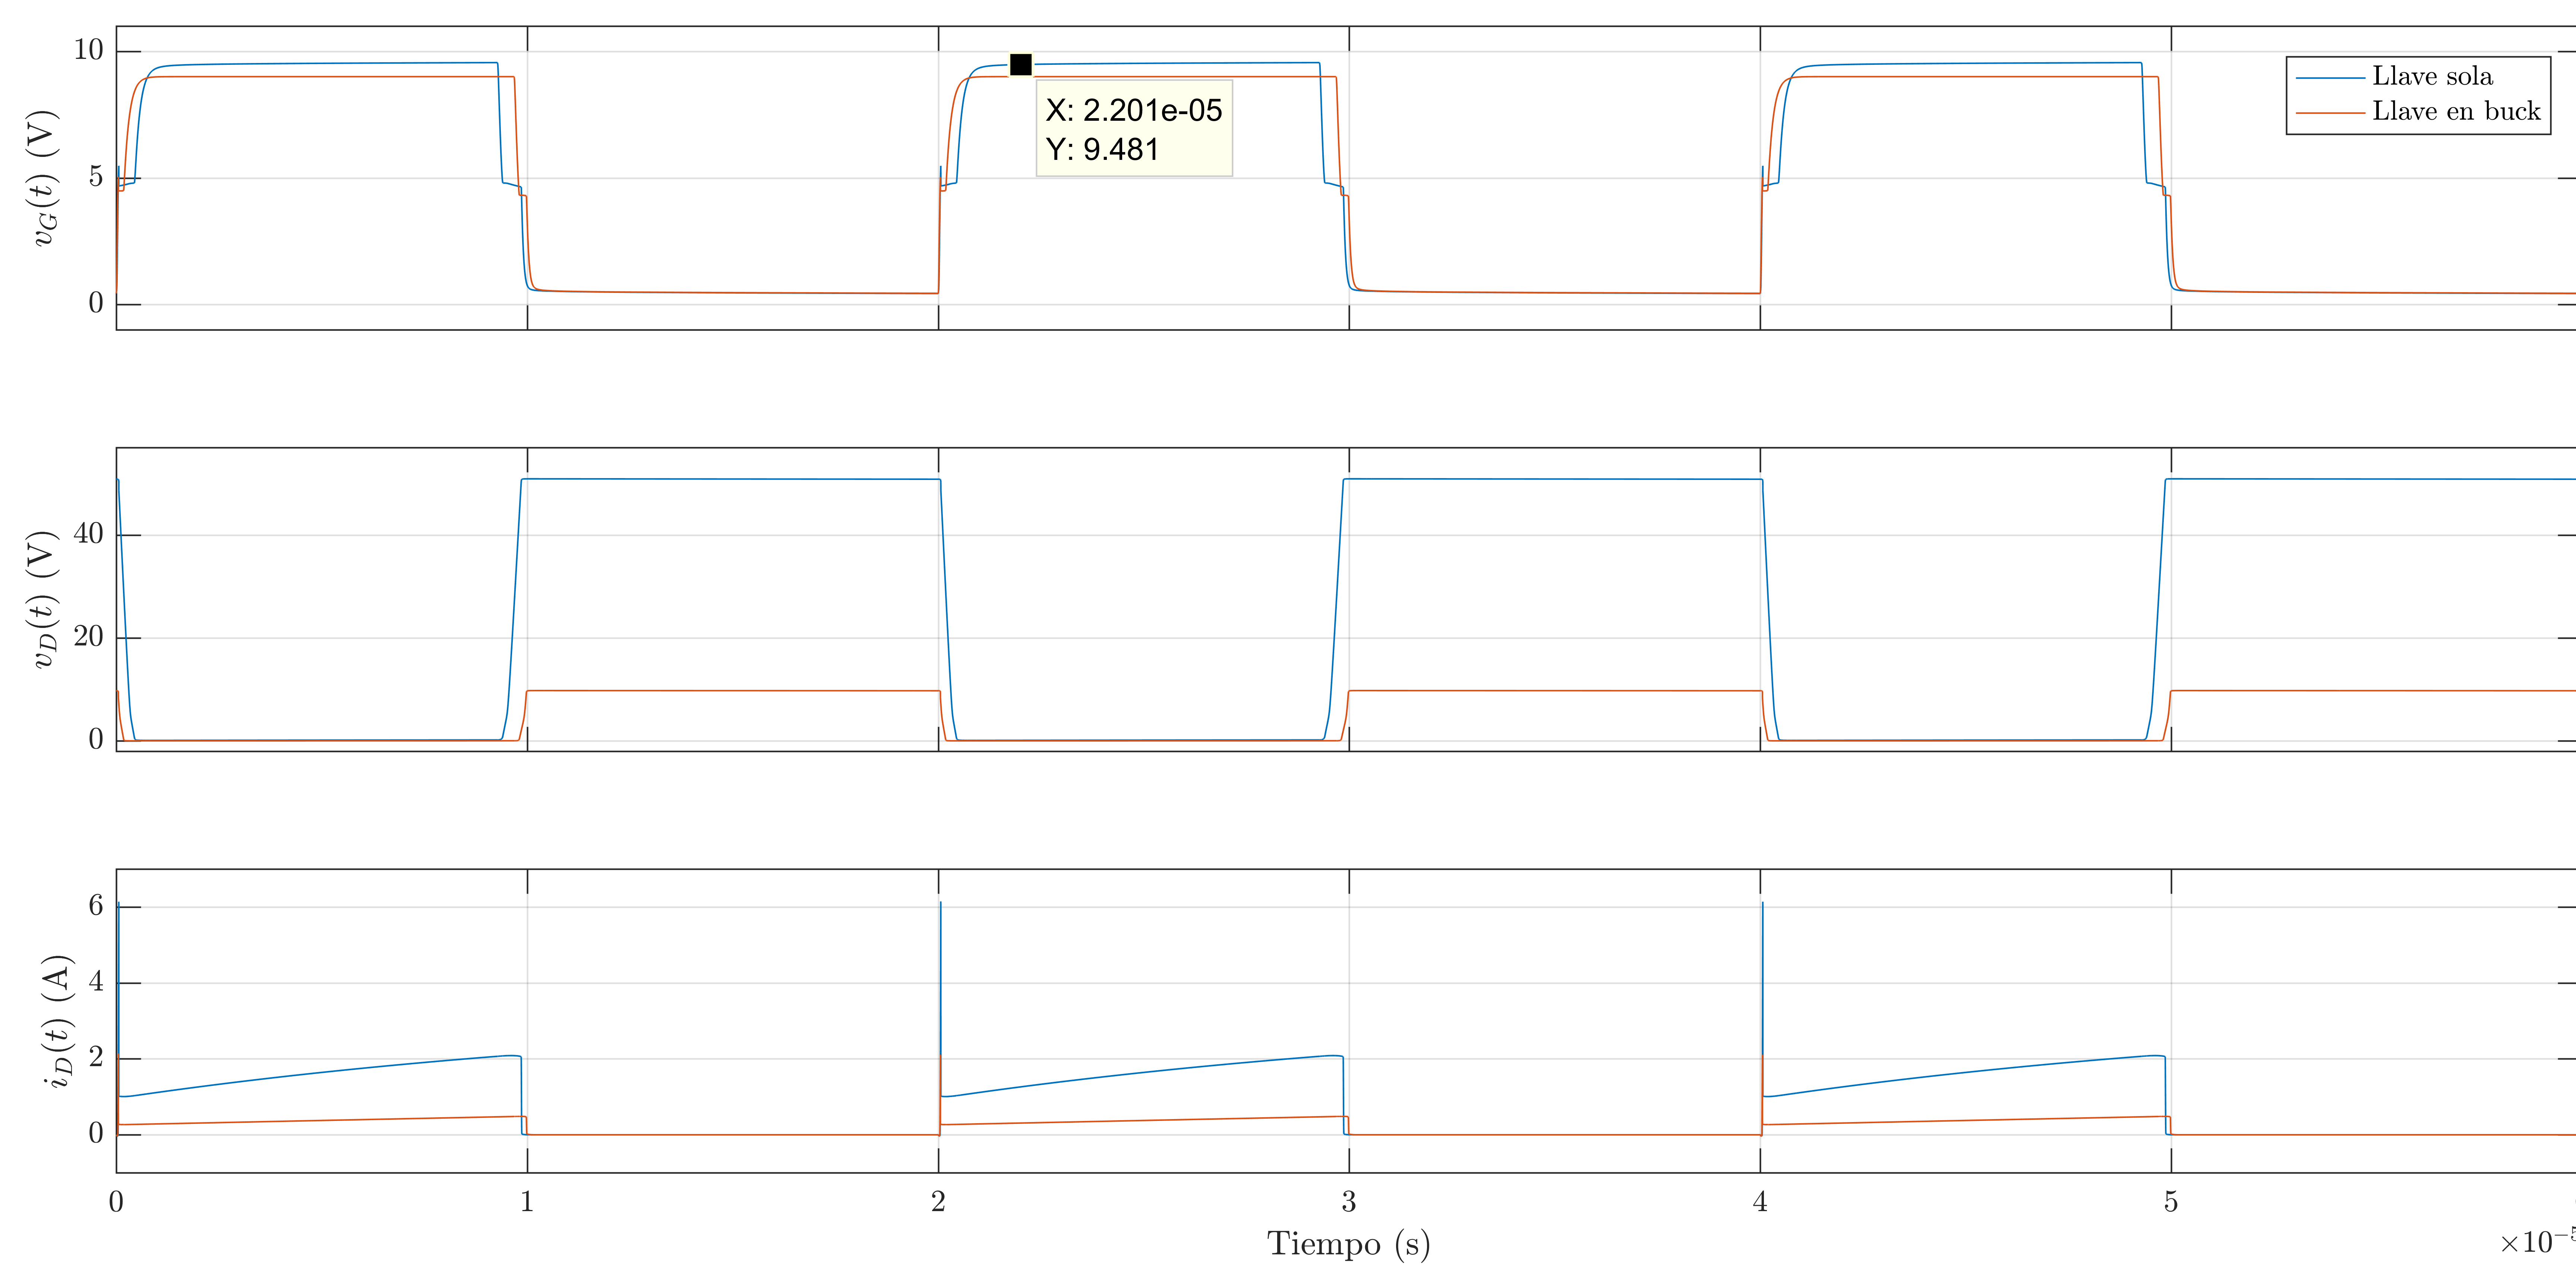
\includegraphics[width=0.75\textwidth]{images/ej3/conmutacion3.png}
		\caption{Curvas simuladas de conmutaci\'on de la llave con y sin la buck: de arriba hacia abajo, tensi\'on de gate, tensi\'on de drain, y corriente de drain.}
		\label{fig:curvas3}
	\end{figure}


\end{document}